% Тут используется класс, установленный на сервере Papeeria. На случай, если
% текст понадобится редактировать где-то в другом месте, рядом лежит файл matmex-diploma-custom.cls
% который в момент своего создания был идентичен классу, установленному на сервере.
% Для того, чтобы им воспользоваться, замените matmex-diploma на matmex-diploma-custom
% Если вы работаете исключительно в Papeeria то мы настоятельно рекомендуем пользоваться
% классом matmex-diploma, поскольку он будет автоматически обновляться по мере внесения корректив
%

% По умолчанию используется шрифт 14 размера. Если нужен 12-й шрифт, уберите опцию [14pt]
\documentclass[14pt]{matmex-diploma-custom}
%\documentclass[14pt]{matmex-diploma-custom}

\begin{document}
% Год, город, название университета и факультета предопределены,
% но можно и поменять.
% Если англоязычная титульная страница не нужна, то ее можно просто удалить.
\filltitle{ru}{
    chair              = {Программная инженерия},
    title              = {Цифровая обработка изображений в микроскопии},
    % Здесь указывается тип работы. Возможные значения:
    %   coursework - Курсовая работа
    %   diploma - Диплом специалиста
    %   master - Диплом магистра
    %   bachelor - Диплом бакалавра
    type               = {diploma},
    position           = {студента},
    group              = 471,
    author             = {Кутуев Владимир Александрович},
    supervisorPosition = {доц.,\,к.т.н.},
    supervisor         = {Ю.\,В. Литвинов},
    % reviewerPosition   = {ст. преп.},
    % reviewer           = {Привалов А.\,И.},
    consultPosition   = {ст. преп.},
    consult           = {Я.\,А. Кириленко},
    % chairHeadPosition  = {д.\,ф.-м.\,н., профессор},
    % chairHead          = {Хунта К.\,Х.},
%   university         = {Санкт-Петербургский Государственный Университет},
%   faculty            = {Математико-механический факультет},
%   city               = {Санкт-Петербург},
%   year               = {2013}
}

\maketitle
\tableofcontents
% У введения нет номера главы
\section*{Введение}

% С развитием технологий оптической микроскопии стоимость простых микроскопов стала достаточно низкой для массового использования дома и в образовательных учреждениях. 
В оптической микроскопии один из главных факторов получения резких изображений --- оптическая система микроскопа, которая непосредственно влияет на его разрешающую способность. Но улучшение оптики микроскопа связано с материальными затратами. Цифровая обработка позволяет повысить качество получаемых изображений, без замены оптики. Также получить максимально резкое изображение исключительно средствами оптики микроскопа не всегда возможно. У объёмных препаратов при большом увеличении с помощью микроскопа можно сфокусироваться только на ограниченные области исследуемого объекта, об этой проблеме говорится в статьях <<Complex wavelets for extended depth-of-field: A new method for the fusion of multichannel microscopy images>>~\cite{MethodForTheFusion}, <<FocusALL: Focal Stacking of Microscopic Images Using Modified Harris Corner Response Measure>>~\cite{ModifiedHarrisCorner}, <<Extended depth-of-field via focus stacking and graph cuts>>~\cite{ExtendedDepthOfField}. Рассеянный свет из областей, находящихся вне зоны фокуса, влечёт появление различных артефактов, которые влияют на чёткость изображения, эта проблема рассматривается в статье <<Blurring-Effect-Free CNN Network of Structural Edge for Focus Stacking>>~\cite{BlurringEffectFree}. Цифровая обработка позволяет решить эти проблемы. Примерами инструментов цифровой обработки, позволяющих решать такие проблемы, являются Zerene Stacker~\cite{ZereneStacker}, Helicon Focus~\cite{HeliconFocus}, Extended Depth of Field Plugin for ImageJ~\cite{ExtendedDepthOfField}, Affinity Photo~\cite{Affinity}, Adobe Photoshop~\cite{Photoshop}.
\par
Особый интерес в микроскопии представляет изучение подвижных микроорганизмов, поэтому цифровая обработка должна иметь высокую производительность, чтобы обрабатывать видео в реальном времени с низкой задержкой.
\par
За последние несколько лет мобильные платформы приобрели большую популярность, такой вывод можно сделать на основе статистики анализа web-трафика порталом StatCounter~\cite{StatCounter}. Также интерес к мобильным платформам повышает наличие у большинства смартфонов камер, которые можно использовать для захвата изображений с микроскопа. В статье <<Mobile Phone Based Clinical Microscopy for Global Health Applications>>~\cite{GlobalHealthApplications} приведён пример использования сотового телефона для обработки изображений со специальной оптической системы для детектирования малярии в крови. В статье <<Quantitative Imaging with a Mobile Phone Microscope>>~\cite{QuantImage} было показано, что с использованием камер современных смартфонов можно захватывать видео без значительной потери разрешающей способности. Однако на данный момент, все текущие решения в области цифровой обработки информации с микроскопа реализованы для desktop платформы. Поэтому интерес представляет разработка кроссплатформенного решения, которое должно поддерживать как desktop-платформы, так и основные мобильные --- Android и iOS.

\section{Постановка задачи}
Цель работы --- разработать кроссплатформенную библиотеку для обработки набора кадров, снятых с использованием оптического микроскопа, которая позволит получать изображение более высокого качества. Также библиотека должна быть расширяемой для внедрения других алгоритмов улучшения получаемого изображения. Важно, чтобы решение работало быстро, сохраняя качество, удовлетворяющее человека. Для достижения цели были поставлены следующие задачи.
\begin{enumerate}
    \item Реализовать систему для визуального сравнения результатов работы алгоритмов обработки набора кадров. 
    \item Провести опрос, какие из алгоритмов выполняют задачу лучше.
    \item Создать прототип для замера скорости работы алгоритмов.
    \item Реализовать кроссплатформенную мобильную библиотеку.
    \item Провести тестирование библиотеки на desktop платформе, iOS, Android.
\end{enumerate}


\section{Фокус-стекинг(Focus stacking)}
Для получения резкого изображения плоского препарата достаточно подобрать расстояние фокусировки, при котором всё изображение попадает в фокус. Однако сделать это с объёмными объектами нельзя. Глубина резкости микроскопа ограничена, и сфокусированными получаются только определённые области препарата. Для решения этой проблемы применяется техника фокус-стекинга: производится захват серии изображений при разных уровнях фокуса, затем для каждого изображения определяются наиболее сфокусированные участки. Из них формируется изображение, в котором все области попадают в фокус (рис.\ref{focus_stacking1}).

\begin{figure}[h]
    \centering
    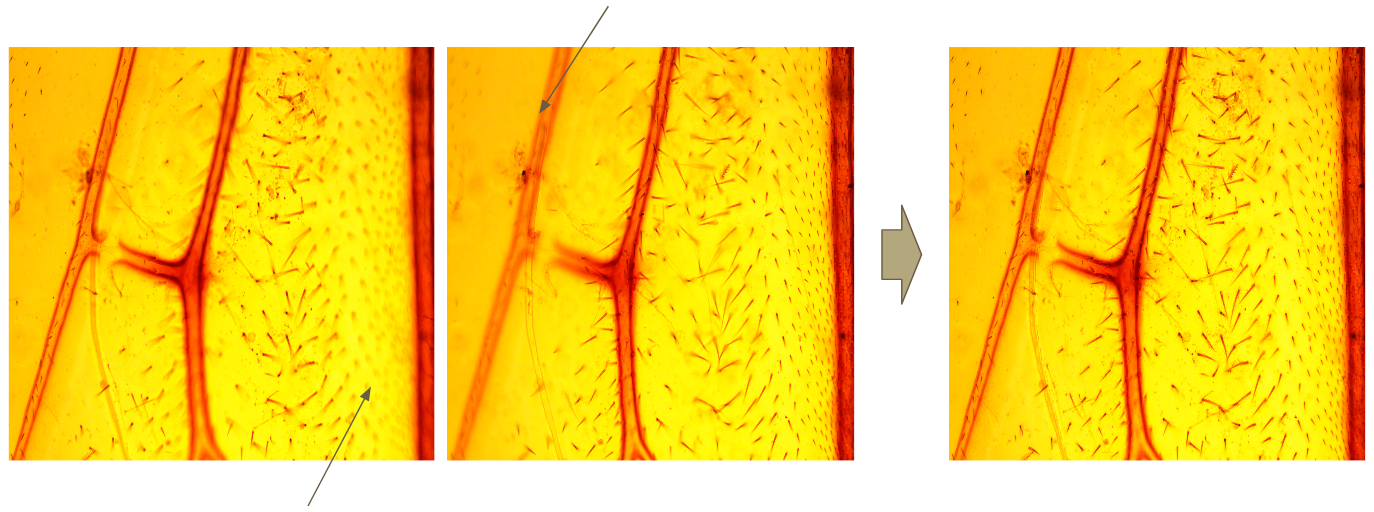
\includegraphics[width=1.0\textwidth]{figures/fs1.png}
    \caption{Фокус-стекинг}
    \label{focus_stacking1}
\end{figure}

\section{Операторы фокусной меры}
Так как было выявлено требование высокго быстродействия обработки серии изображений, то необходимо отбирать наиболее сфокусированные изображения, чтобы сократить время работы алгоритма фокус-стекинга и уменьшить количества шума в итоговом изображении. Для определения четкости изображения используются операторы фокусной меры (Objective functions). Они делятся на несколько групп:
\begin{itemize}
    \item основанные на градиенте;
    \item основанные на операторе Лапласа;
    \item основанные на вейвлет преобразованиях;
    \item статистические;
    \item смешанные.
\end{itemize}

Обзор различных операторов и сравнение их производительности при различных аспектах: зашумлённость изображений, размер окна оператора --- приведены в статье <<Analysis of focus measure operators in shape-from-focus>>~\cite{MeasureOperators}.

В работе <<Automated focusing in bright-field microscopy for tuberculosis detection>>~\cite{BestOperators} было рассмотрено применение операторов фокусной меры для автоматической фокусировки в микроскопии. В статье предлагается использовать операторы фокусной меры для выбора самого сфокусированного кадра среди снятых и приводится сравнение этих операторов по качеству работы, точности и скорости поиска фокуса с их помощью.

Опираясь на изученные научные статьи, для реализации были выбраны операторы:
\begin{itemize}
    \item Laplacian Variance; 
    \item Tenengrad operator;
    \item Vollath F4;
    \item Modified Laplacian.
\end{itemize}
Выбор сделан с учетом необходимости получения высокопроизводительных операторов, приспособленных к работе с изображениями в области микроскопии.

\section{Повышение качества кадров}
\subsection{Удаление пыли}

При получении изображений с микроскопа можно столкнуться с проблемой наличия в кадре объектов, которые не являются частью изучаемого препарата --- пыли или капель. Чтобы решить эту проблему, можно по расфокусированному содержащему пыль изображению создать маску (рис. \ref{dust_map1}), по которой пыль будет удаляться в обрабатываемых изображениях (рис. \ref{dust_filtering1}).

\begin{figure}[h]
    \centering
    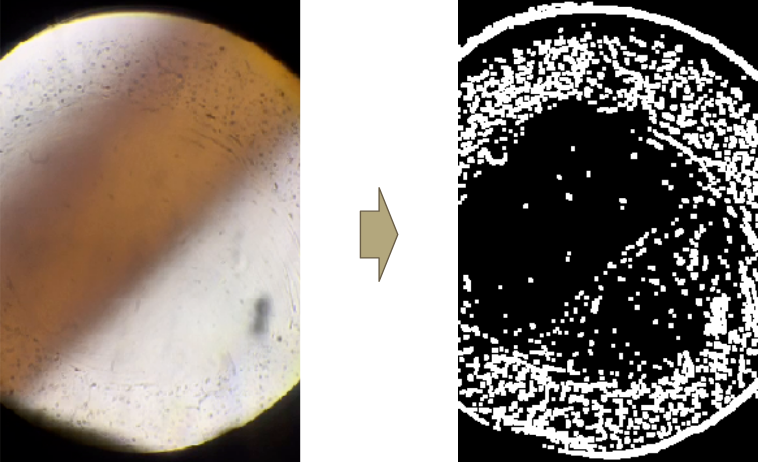
\includegraphics[width=1.0\textwidth]{figures/dust1.png}
    \caption{Создание маски}
    \label{dust_map1}
\end{figure}

\newpage

\begin{figure}[h]
    \centering
    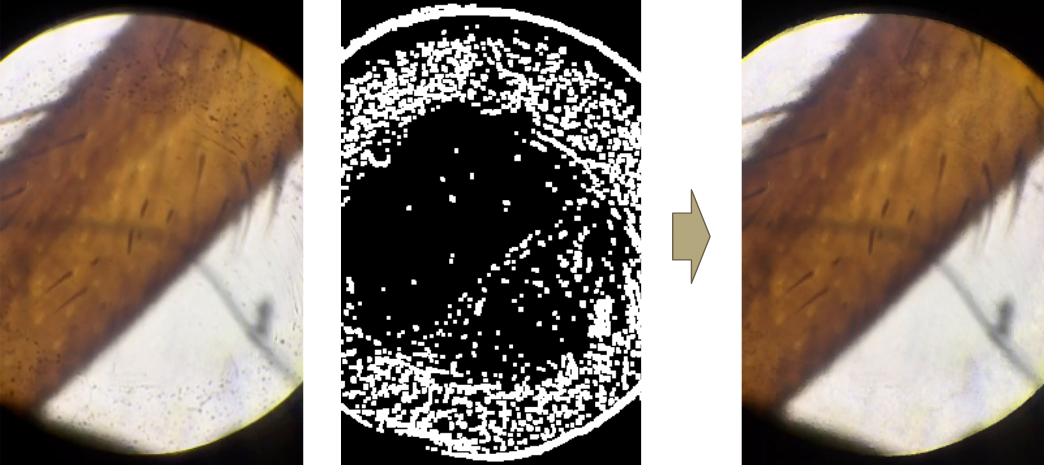
\includegraphics[width=0.95\textwidth]{figures/dust2.png}
    \caption{Удаление пыли}
    \label{dust_filtering1}
\end{figure}


\subsection{Деконволюция}
Рассеянный свет из областей, находящихся вне зоны фокуса, ниже или выше фокальной плоскости, становится причиной появления блеска, искажения и нерезкости при получении изображений. Деконволюция –-- способ обработки изображения, позволяющий избавиться от этих нежелательных эффектов. На Рис.\ref{deconvolution1} представлен результат алгоритма деконволюции <<Richardson–Lucy with Total Variation>>~\cite{RLTV}. Этот пример показывает, что этот метод позволяет значительно улучшить полученное изображение.

\begin{figure}[h]
    \centering
    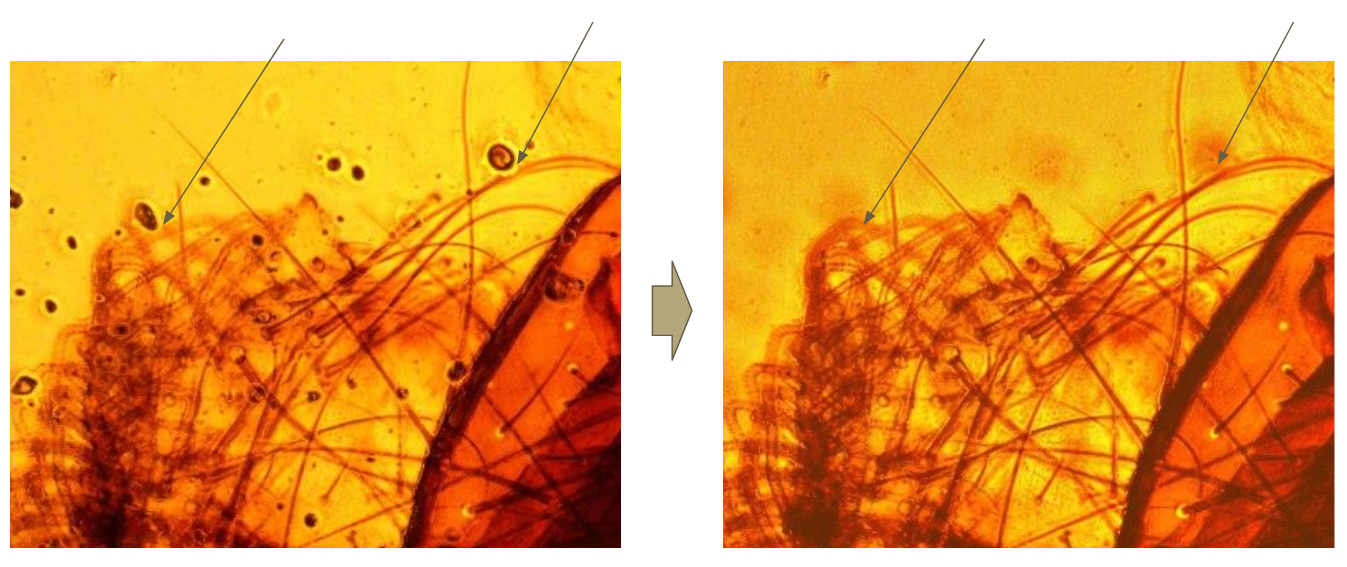
\includegraphics[width=.95\textwidth]{figures/deconvolution1.png}
    \caption{Деконволюция}
    \label{deconvolution1}
\end{figure}

\newpage
Однако деконволюция --- операция, требующая достаточно много времени, поэтому было решено провести исследование, как деконволюция влияет на значение оператора фокусной меры. Рис. \ref{deconvolution2} показывает значение оператора фокусной меры, получаемой на каждом кадре из видео. Можно заметить, что после деконволюции кадры становятся более сфокусированными, но тенденции изменения значения сохраняются на протяжении видео. Дальнейшее исследование должно ответить на вопрос: можно ли отказаться от этой операции на этапе отбора кадров и применять её  только к результату фокус-стекинга.

\begin{figure}[h]
    \centering
    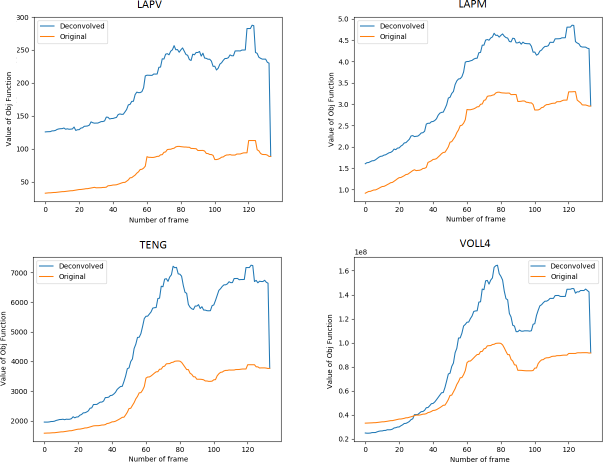
\includegraphics[width=1.0\textwidth]{figures/deconvolution2.png}
    \caption{Значение оператора фокусной меры до и после деконволюции}
    \label{deconvolution2}
\end{figure}


\section{Сравнение результатов работы алгоритмов}

Важная часть работы --- выбор алгоритмов, результат работы которых будет удовлетворительным для человеческого глаза. Отсутствие существенных отличий в результатах нескольких алгоритмов позволит сфокусироваться на более быстрых. Поэтому нужен удобный инструмент для сравнения результатов. Так как целевые устройства --- смартфоны, то этот инструмент должен поддерживать мобильные платформы. Для данных целей разработано web-приложение, удовлетворяющее этим требованиям. На Рис.\ref{comparation1} и Рис.\ref{comparation2} показан его интерфейс. Он разрабатывался с учётом необходимости переключиться между любыми алгоритмами, чтобы сразу увидеть разницу между полученными результатами. Также в этом приложении предусмотрена автоматическая отправка информации о том, результат какого из алгоритмов понравился опрашиваемому больше. 
% При тестировании этого приложения было замечено, что различия в результатах на экране смартфона менее заметны, чем на мониторе компьютера. Поэтому был добавлена отправка информации о размерах экрана, на котором проводилось сравнение.

\begin{figure}[h]
    \centering
    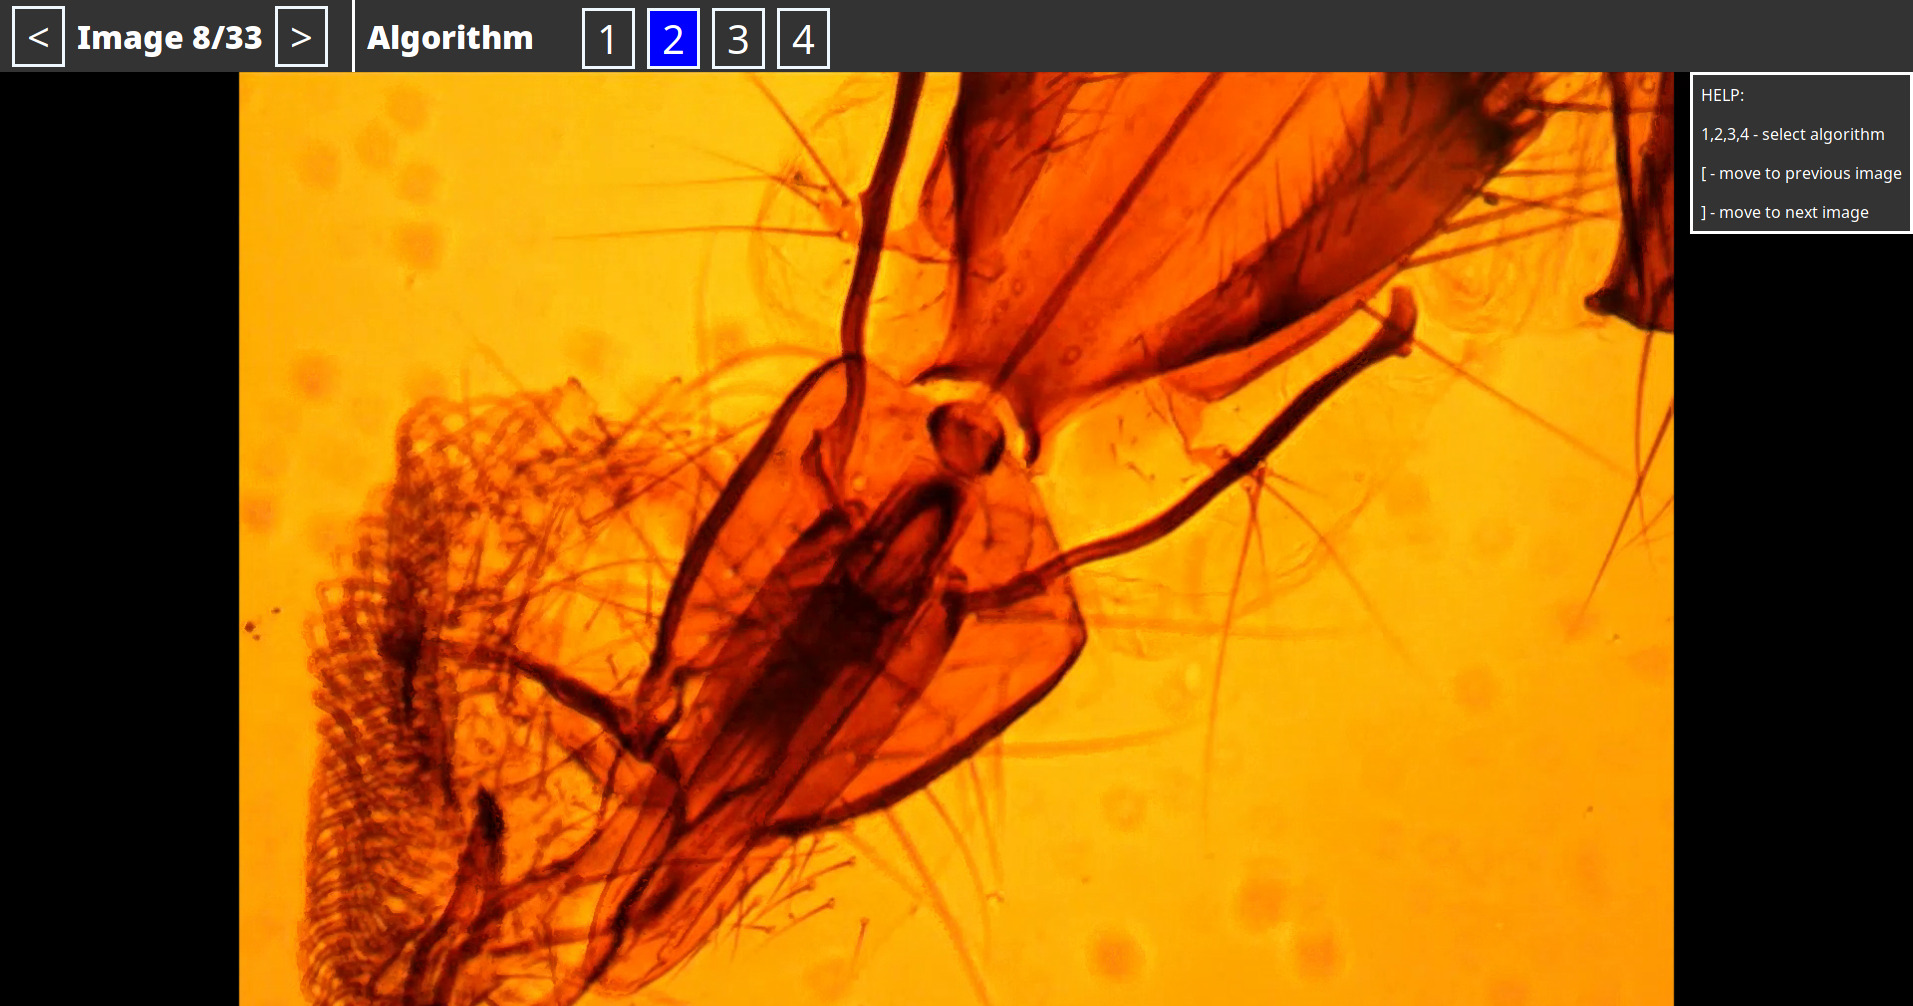
\includegraphics[width=1.0\textwidth]{figures/comparasion1.jpg}
    % \caption{Desktop}
    \caption{Desktop интерфейс}
    \label{comparation1}
\end{figure}

\newpage

\begin{figure}[h]
    \begin{subfigure}{.25\textwidth}
        \centering
        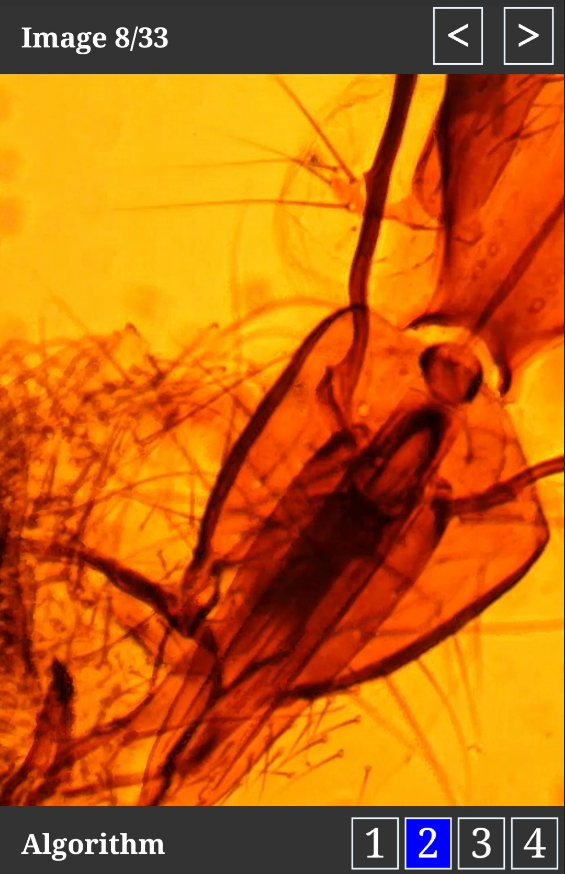
\includegraphics[width=.9\linewidth,height=6cm]{figures/comparasion2.png}
        % \caption{Portrait}
        \caption{Портретная ориентация}
        \label{fig:sfig1}
    \end{subfigure}
    \begin{subfigure}{.75\textwidth}
        \centering
        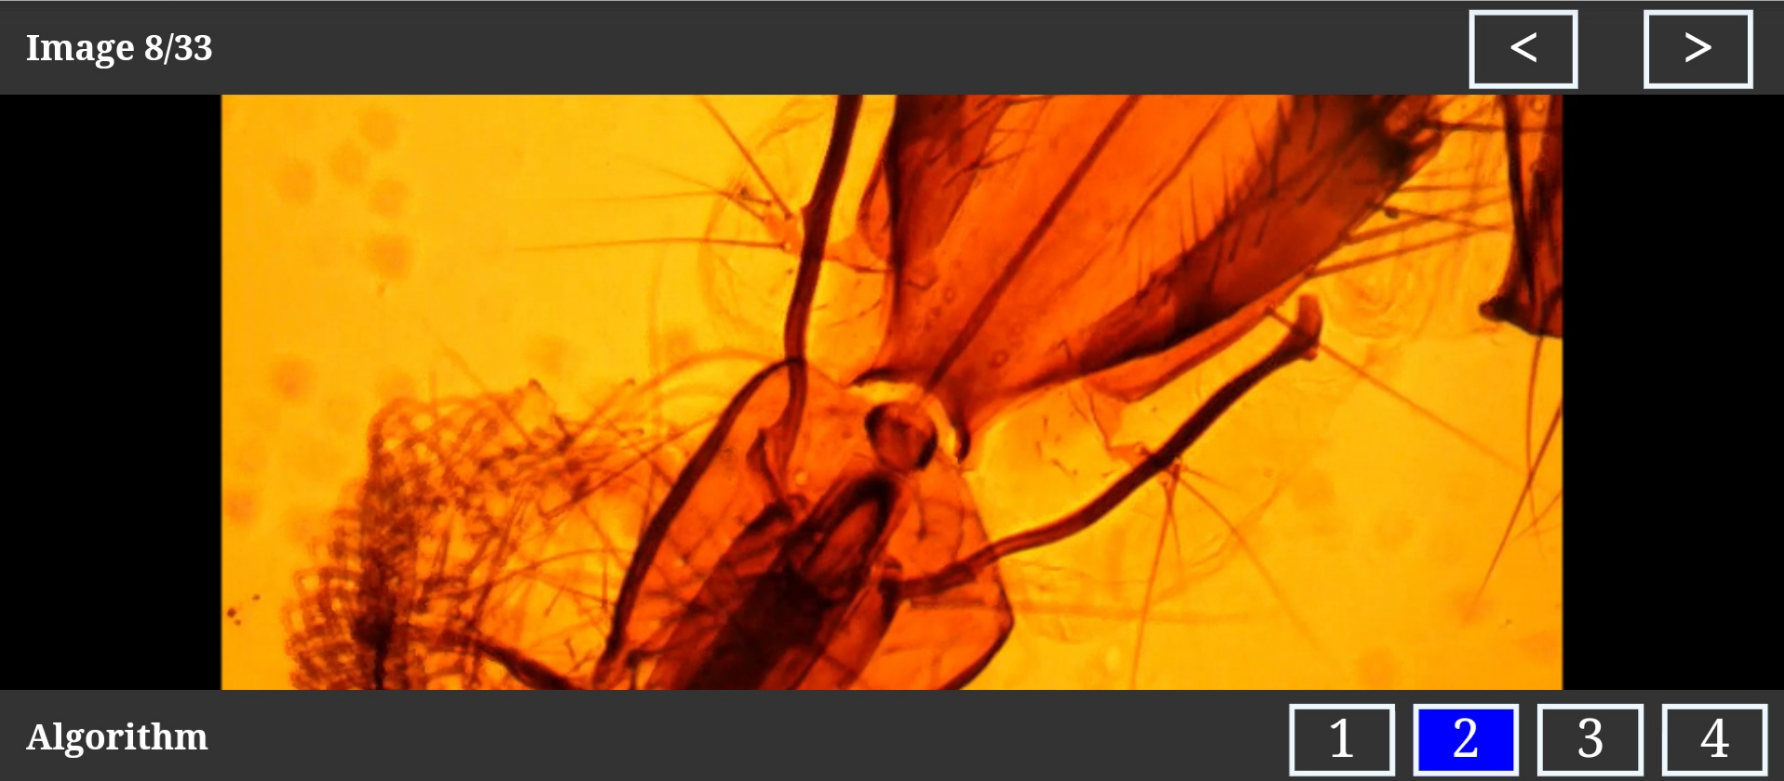
\includegraphics[width=.9\linewidth,height=6cm]{figures/comparasion3.png}
        % \caption{Landscape}
        \caption{Альбомная ориентация}
        \label{fig:sfig2}
    \end{subfigure}
    % \caption{Mobile}
    \caption{Мобильный интерфейс}
    \label{comparation2}
\end{figure}

\section{Реализация}

% Djinni для сокращения цикла разработки -- исправить Djinni файл, описывающий интерфейсы, дописать туда код, пересобрать.
%
% Для получения класса реализующего библиотеку используется паттерн фабричный метод(билдер), которому в аргументы передаются опции описывающие алгоритмы, которые он должен применять к последовательности изображений. Такой подход был выбран, для скорости прототипирования
% 
Так как важным требованием к создаваемой библиотеке является быстродействие, то было принято решение реализовывать её на языке программирования C++, а для её использования из-под мобильных платформ воспользоваться инструментом Djinni~\cite{Djinni}.
% Использовать данный инструмент было решено, чтобы сократить 
Код на C++ компилируется под нужные платформы, а с помощью Djinni генерируются интерфейсы взаимодействия кода библиотеки с платформенно-ориентированным кодом на Java и Objective-C на Android и iOS. 
\par
В разрабатываемой библиотеке при обработке потока входных кадров и реализации алгоритмов фокус-стекинга и операторов фокусной меры было решено воспользоваться функциональностью, предоставляемой библиотекой OpenCV~\cite{OpenCV}.

% % У заключения нет номера главы
\section*{Заключение}
% В данный момент в библиотеке реализованы:
В ходе работы над проектом были достигнуты следующие результаты.
\begin{enumerate}
    \item Создано web-приложение для визуального сравнения результатов работы алгоритмов. 
    \item В кроссплатформенной библиотеке реализованы:
        \begin{itemize}
            \item оператор фокусной меры Tenengrad;
            \item алгоритм удаления пыли;
            \item алгоритм фокус-стекинга, основанный на одиночных пикселях.
        \end{itemize}
\end{enumerate}

\par
Основные направления дальнейшей работы:
\begin{itemize}
    \item провести опрос, чтобы выявить наиболее подходящие алгоритмы для внедрения в библиотеку;
    \item провести замеры скорости работы алгоритмов;
    \item реализовать фильтрацию кадров с одинаковыми областями фокуса;
    \item реализовать выбранные алгоритмы фокус-стекинга;
    \item реализовать выбранные операторы фокусной меры;
    \item реализовать алгоритм деконволюции;
    \item провести тестирование библиотеки на desktop платформе, iOS, Android.
\end{itemize}

\setmonofont[Mapping=tex-text]{CMU Typewriter Text}
\bibliographystyle{ugost2008ls}
\bibliography{diploma.bib}
\end{document}
